\section{Metodología}
\label{sec:metodologia}
La metodología adoptada para el diseño, ejecución y evaluación de la simulación de la propagación de ransomware se estructuró de forma cronológica en fases consecutivas, orientadas a garantizar el rigor científico y la reproducibilidad del experimento. Se detalla a continuación el diseño conceptual basado en agentes cognitivos BDI, la carga de datos georreferenciados, el motor matemático de infección y las reglas lógicas que gobiernan el modelo.

\subsection{Concepción del Modelo y Definición de Agentes}
El modelo se fundamenta en el paradigma de sistemas multiagente (MAS) para representar de forma distribuida e individualizada la infraestructura de la red universitaria. Se definieron tres especies principales de agentes en GAML:
\begin{enumerate}
    \item \textbf{Agente Sala (Spatial Agent):} Representa el entorno físico o espacial de los laboratorios. No posee lógica activa en la red, pero establece las fronteras geométricas para la delimitación de los clústeres de computadoras. Su único atributo es su nombre identificativo (por ejemplo, Sala 1, Sala 2).
    \item \textbf{Agente Nodo (Network Computer Agent):} Representa a los dispositivos activos interconectados. Los agentes de esta especie poseen atributos específicos de red y seguridad. Se subdividen dinámicamente según su función lógica en:
    \begin{itemize}
        \item \textit{Internet:} Actúa como el origen WAN y paciente cero de la amenaza.
        \item \textit{Firewall:} Cortafuegos perimetral encargado de filtrar el tráfico entrante.
        \item \textit{Switch:} Concentrador central que enruta la comunicación física entre salas.
        \item \textit{Server:} Servidor local de recursos compartidos de la red universitaria.
        \item \textit{PC:} Modela las estaciones de trabajo de los estudiantes dentro de cada laboratorio.
    \end{itemize}
    Los atributos de control definidos para cada agente Nodo son:
    \begin{itemize}
        \item $id$: Identificador único entero del nodo.
        \item $nombre$: Cadena de texto identificativa.
        \item $infected$: Booleano que indica si el equipo ha sido comprometido por el ransomware.
        \item $secured$: Booleano que indica si el equipo ha recibido parches e inmunización.
        \item $isolated$: Booleano que indica si el equipo ha sido aislado lógicamente (en cuarentena).
        \item $open\_ports$: Lista de puertos TCP/UDP abiertos (por ejemplo, [445, 3389, 80]).
        \item $patch\_level$: Nivel entero entre $0$ y $100$ que representa la actualización del sistema.
        \item $cooldown$: Contador de ciclos de espera entre intentos de propagación.
    \end{itemize}
    \item \textbf{Agente Conexión (Link Agent):} Modela los enlaces físicos o lógicos bidireccionales de comunicación de datos. Conserva la geometría exacta de las líneas físicas y vincula un agente origen con un agente destino.
\end{enumerate}

Para dotar de racionalidad local a las estaciones de trabajo ante incidentes de seguridad, el agente Nodo implementa la arquitectura cognitiva BDI (Belief-Desire-Intention) propuesta por Rao y Georgeff \cite{rao1995bdi}. Sus componentes lógicos se detallan en la Tabla \ref{tab:componentes_bdi}.

\begin{table}[htbp]
\caption{Componentes de la Arquitectura BDI del Agente Computadora}
\label{tab:componentes_bdi}
\begin{center}
\footnotesize
\begin{tabular}{|p{0.20\columnwidth}|p{0.25\columnwidth}|p{0.39\columnwidth}|}
\hline
\textbf{Componente} & \textbf{Definición Lógica} & \textbf{Representación en GAML} \\ \hline
\textbf{Beliefs} \newline (Creencias) & Percepción local del estado de red y su propia seguridad & 
\texttt{bel\_amenaza\_cercana}, \newline 
\texttt{bel\_soy\_vulnerable}, \newline 
\texttt{bel\_riesgo}, \newline 
\texttt{bel\_red\_comprometida} \\ \hline
\textbf{Desires} \newline (Deseos) & Objetivos fundamentales del agente & 
\texttt{des\_sobrevivir}, \newline 
\texttt{des\_infectar}, \newline 
\texttt{des\_aislarse}, \newline 
\texttt{des\_parchear} \\ \hline
\textbf{Intentions} \newline (Intenciones) & Planes comprometidos de acción inmediata & 
\texttt{normal}, \texttt{spread}, \newline 
\texttt{patch}, \texttt{isolate}, \newline 
\texttt{isolated} \\ \hline
\end{tabular}
\end{center}
\end{table}

El ciclo de transiciones lógicas de los estados de un agente Nodo se ilustra en la Figura \ref{fig:estados_agente}.

\begin{figure}[htbp]
\centering
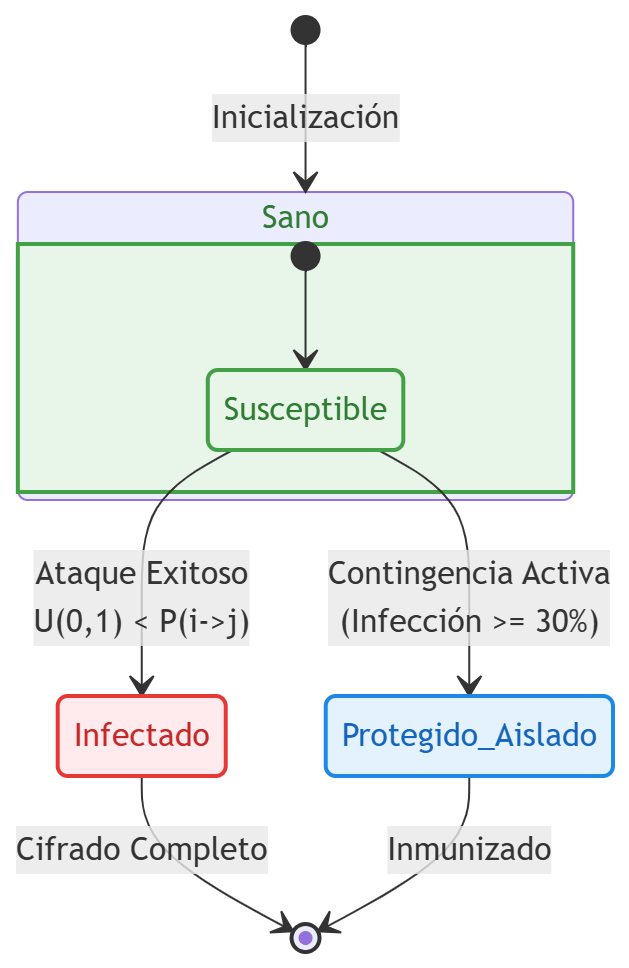
\includegraphics[width=0.85\columnwidth]{assets/estados_agente.png}
\caption{Diagrama de transición de estados de un agente Nodo en la simulación (FSM).}
\label{fig:estados_agente}
\end{figure}

\subsection{Ciclo de Ejecución Cognitivo BDI}
En cada paso de la simulación, cada agente que representa a un host de red ejecuta secuencialmente un ciclo estructurado en cuatro fases:
\begin{enumerate}
    \item \textbf{Fase de Percepción (\texttt{BDI\_}\allowbreak\texttt{perception}):} El agente Nodo examina su vecindad topológica inmediata a través de los agentes Conexión. Determina la cantidad de vecinos infectados y actualiza su estado cognitivo:
    \begin{itemize}
        \item \texttt{bel\_vecinos\_}\allowbreak\texttt{infectados} $\leftarrow$ número de hosts adyacentes comprometidos.
        \item \texttt{bel\_amenaza\_}\allowbreak\texttt{cercana} $\leftarrow$ \texttt{true} si al menos un vecino está infectado.
        \item \texttt{bel\_}\allowbreak\texttt{riesgo} $\leftarrow$ \texttt{bel\_vecinos\_}\allowbreak\texttt{infectados} $\times 25.0$ (rango $0-100$).
        \item \texttt{bel\_soy\_}\allowbreak\texttt{vulnerable} $\leftarrow$ \texttt{true} si el puerto 445 está abierto y su \texttt{patch\_}\allowbreak\texttt{level} $< 50$.
        \item \texttt{bel\_red\_}\allowbreak\texttt{comprometida} $\leftarrow$ \texttt{true} si la tasa de infección global supera el $50\%$.
    \end{itemize}
    \item \textbf{Fase de Deliberación (\texttt{BDI\_}\allowbreak\texttt{deliberation}):} Los deseos del agente se activan en función de sus creencias actualizadas. El deseo de sobrevivir (\texttt{des\_}\allowbreak\texttt{sobrevivir}) permanece siempre activo. Si el nodo está comprometido, activa el deseo de infectar (\texttt{des\_}\allowbreak\texttt{infectar}). Si percibe amenaza cercana o red comprometida, activa el deseo de aislarse (\texttt{des\_}\allowbreak\texttt{aislarse}). Si es vulnerable y percibe amenaza, activa el deseo de parchear (\texttt{des\_}\allowbreak\texttt{parchear}).
    \item \textbf{Fase de Planificación (\texttt{BDI\_}\allowbreak\texttt{planning}):} El agente selecciona una única intención de acción a ejecutar en el ciclo. Dado que pueden surgir deseos en conflicto, la toma de decisiones se rige por la jerarquía de prioridades descrita en la Tabla \ref{tab:prioridades_bdi}.
    \item \textbf{Fase de Ejecución (\texttt{BDI\_}\allowbreak\texttt{execute}):} El agente ejecuta las acciones asociadas a la intención seleccionada:
    \begin{itemize}
        \item \textit{isolated} / \textit{isolate}: El nodo se marca como aislado y queda bloqueado para cualquier tráfico o propagación de malware.
        \item \textit{patch}: Incrementa el \texttt{patch\_}\allowbreak\texttt{level} de forma autónoma a razón de $10$ unidades por ciclo hasta alcanzar el umbral seguro de $50$.
        \item \textit{spread}: Invoca la función \texttt{spread\_}\allowbreak\texttt{action()} para escanear y tratar de infectar a un vecino.
        \item \textit{normal}: El agente permanece en estado inactivo u operativo estándar.
    \end{itemize}
\end{enumerate}

\begin{table}[htbp]
\caption{Jerarquía de Prioridades para la Selección de Intenciones}
\label{tab:prioridades_bdi}
\begin{center}
\footnotesize
\begin{tabular}{|c|c|p{0.58\columnwidth}|}
\hline
\textbf{Prioridad} & \textbf{Intención} & \textbf{Condición de Activación en GAML} \\ \hline
1 & \texttt{isolated} & \texttt{isolated = true} \newline (nodo desconectado previamente) \\ \hline
2 & \texttt{isolate} & \texttt{des\_aislarse} $\land$ \texttt{bel\_riesgo} $> 50$ $\land$ \newline \texttt{flip(containment\_threshold / 100)} \\ \hline
3 & \texttt{patch} & \texttt{des\_parchear} $\land$ $\neg$\texttt{infected} \\ \hline
4 & \texttt{spread} & \texttt{des\_infectar} \newline (nodo comprometido activamente) \\ \hline
5 & \texttt{normal} & Estado por defecto (operación estándar) \\ \hline
\end{tabular}
\end{center}
\end{table}

\subsection{Carga e Integración de Datos Georreferenciados (GIS)}
Para dotar al modelo de una fidelidad espacial que refleje una distribución real, se utilizó un Sistema de Información Geográfica (GIS) mediante la herramienta QGIS. En este entorno, se georreferenciaron los planos del pabellón universitario y se trazaron tres capas vectoriales en formato Shapefile:
\begin{itemize}
    \item \textbf{\texttt{sala.shp}:} Contiene los polígonos que delimitan la geometría y ubicación de los laboratorios físicos de computación.
    \item \textbf{\texttt{nodos.shp}:} Contiene las coordenadas puntuales de cada equipo informático, servidor, switch y firewall, junto con sus atributos iniciales cargados en la tabla de datos espaciales.
    \item \textbf{\texttt{conexiones.shp}:} Contiene las líneas poligonales que representan la infraestructura física de cableado estructurado.
\end{itemize}

Durante la inicialización de la simulación en GAMA Platform, el entorno geométrico del mundo se autodefine a partir del contorno o envolvente (\textit{envelope}) de los datos geográficos de los nodos. GAMA instancia dinámicamente cada agente en la posición exacta del espacio tridimensional o bidimensional definida en los archivos shapefiles, creando la topología de red de forma automática al vincular los agentes origen y destino que coincidan con las claves de adyacencia espacial.

\subsection{Motor Matemático de Infección y Propagación Lateral}
La propagación lateral de WannaCry se modeló reproduciendo el ataque mediante escaneos aleatorios de red y la explotación del protocolo SMBv1 en el puerto TCP 445 \cite{enisa2017wannacry}. La transmisión de la amenaza a través de un enlace de red entre un nodo infectado $i$ y un vecino susceptible $j$ se define de forma probabilística.

Se establece una probabilidad base de infección por contacto $p_0 = 0,35$. En cada paso de simulación, la probabilidad final de transmisión de la infección al nodo destino $j$, denotada por $P(i \rightarrow j)$, se modela incorporando las atenuaciones del cortafuegos y el nivel de parcheo local:
\begin{equation}
\begin{split}
    P(i \rightarrow j) = {} & p_0 \cdot (1 - \alpha_{fw} \cdot \delta_{fw}(j)) \cdot \left(1 - \frac{L_{patch}(j)}{150}\right) \\
    & \cdot \mathbb{I}(445 \in \text{Ports}_j) \cdot (1 - \text{isolated}_j)
\end{split}
\label{eq:probability_combined}
\end{equation}
Donde:
\begin{itemize}
    \item $\alpha_{fw} \in [0, 1]$ es el coeficiente de fuerza de mitigación del Firewall.
    \item $\delta_{fw}(j)$ es una función indicadora que vale $1$ si el nodo $j$ es un Firewall, y $0$ en caso contrario.
    \item $L_{patch}(j) \in [0, 100]$ es el nivel de parche actual del nodo receptor.
    \item $\mathbb{I}(445 \in \text{Ports}_j)$ es una función indicadora que vale $1$ si el puerto TCP 445 está abierto en $j$, y $0$ si está cerrado.
    \item $\text{isolated}_j$ es $1$ si el nodo destino está aislado de la red, y $0$ si está conectado.
\end{itemize}

Esta formulación matemática da lugar al espacio de probabilidades resultantes para la propagación que se detalla en la Tabla \ref{tab:espacio_probabilidades}.

\begin{table}[htbp]
\caption{Espacio de Probabilidades Resultantes de Infección}
\label{tab:espacio_probabilidades}
\begin{center}
\begin{tabular}{|c|c|c|p{0.15\columnwidth}|}
\hline
\textbf{Fuerza FW} ($\alpha_{fw}$) & \textbf{Nivel Parche} ($L_{patch}$) & \textbf{Prob. $P$} & \textbf{Escenario Representado} \\ \hline
0,1 & 5\% & $\sim 0,31$ & WannaCry Real (Mayo 2017) \\ \hline
0,7 & 10\% & $\sim 0,10$ & Red con firewall activo \\ \hline
0,9 & 80\% & $\sim 0,002$ & Red bien protegida \\ \hline
1,0 & 100\% & $0,0$ & Red completamente segura \\ \hline
\end{tabular}
\end{center}
\end{table}

La transición efectiva del estado del nodo $j$ de Sano a Infectado en el siguiente ciclo temporal ($t + 1$) se determina simulando una variable aleatoria uniforme continua en el intervalo $[0, 1]$, denotada por $U(0, 1)$. La regla lógica condicional se formaliza en la Ecuación \ref{eq:transition_rule}:
\begin{equation}
    \text{Estado}_j(t+1) = \begin{cases} 
        \text{Infectado} & \text{si } U(0,1) < P(i \rightarrow j) \\ 
        \text{Sano} & \text{en caso contrario} 
    \end{cases}
    \label{eq:transition_rule}
\end{equation}

El flujo algorítmico de evaluación lógica y cálculo probabilístico por cada intento de transmisión lateral se detalla en la Figura \ref{fig:flujo_infeccion}.

\begin{figure}[htbp]
\centering
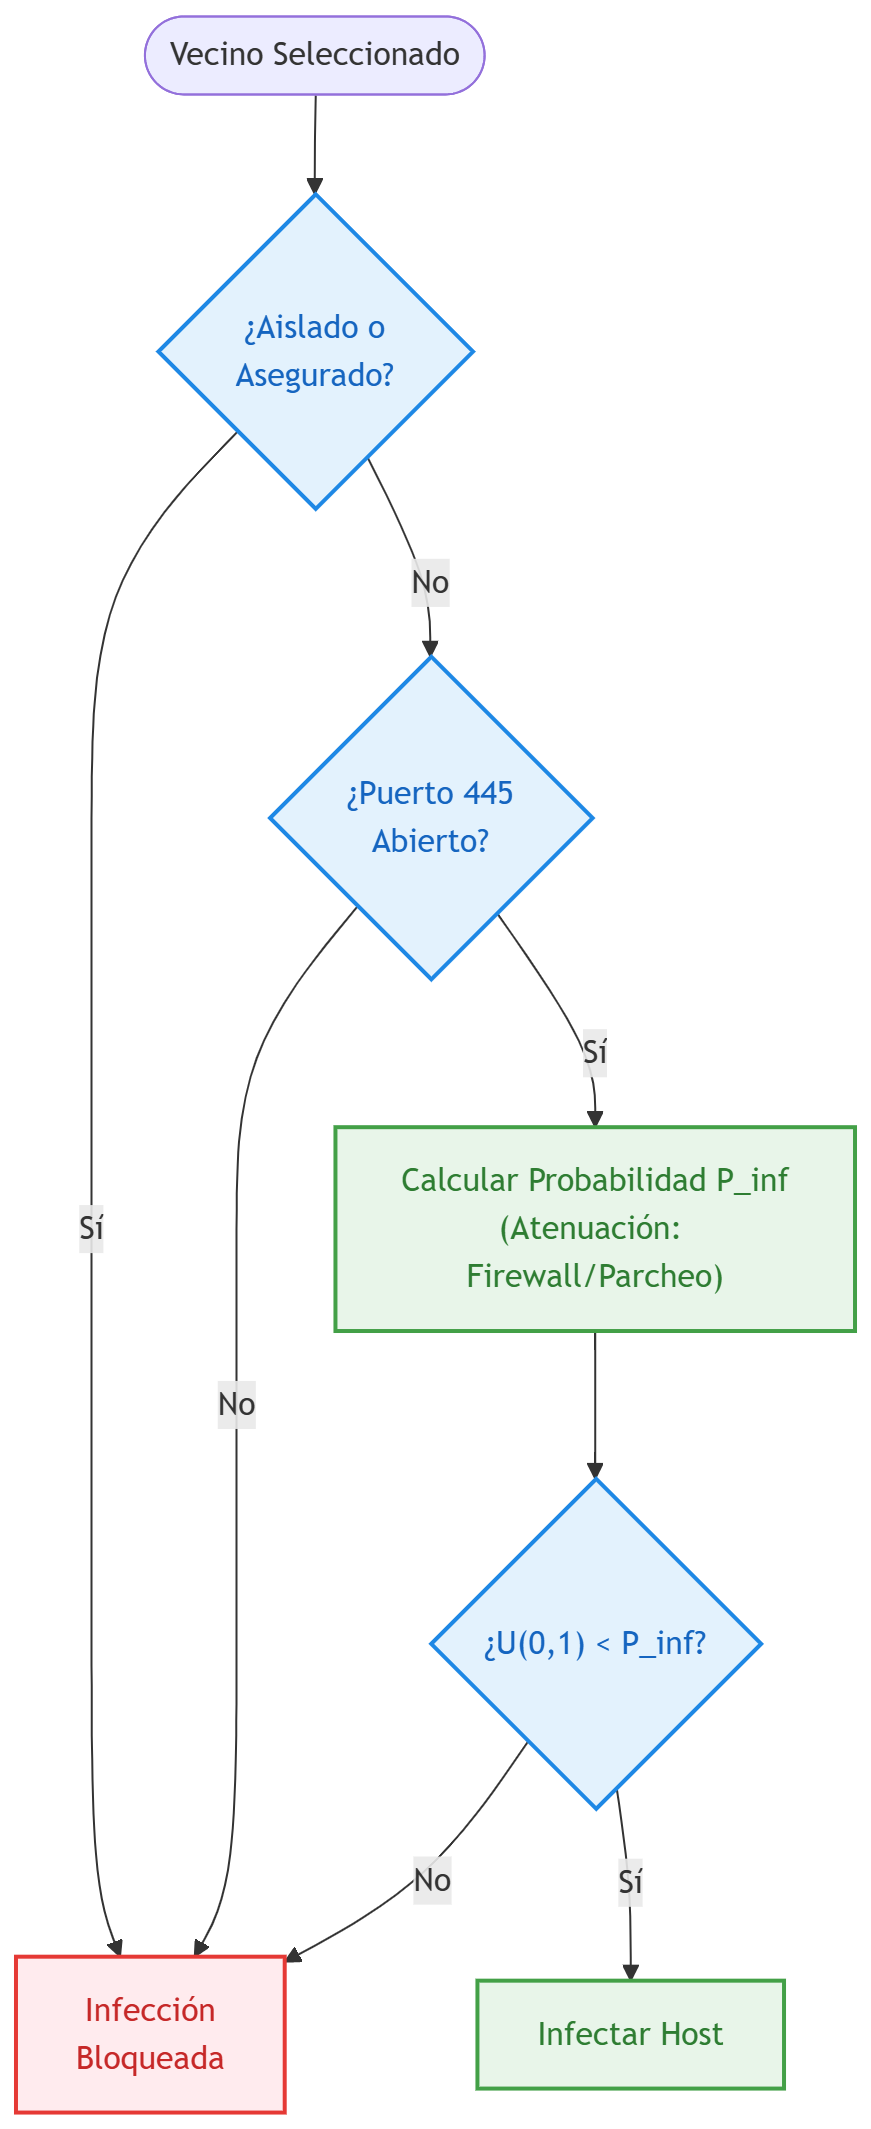
\includegraphics[width=0.9\columnwidth]{assets/flujo_infeccion.png}
\caption{Diagrama de flujo de decisión para el motor de infección probabilístico.}
\label{fig:flujo_infeccion}
\end{figure}

\subsection{Lógica del Protocolo de Contingencia Reactiva y Coordinadores}
Para contrarrestar el avance exponencial de la infección lateral, se diseñó un monitor del sistema de control de red en la simulación. Este monitor actúa bajo dos esquemas de coordinación centralizada global en el bloque \texttt{global} de GAML:

\begin{itemize}
    \item \textbf{Aislamiento Coordinado (\texttt{BDI\_global\_}\allowbreak\texttt{containment}):} En cada ciclo de simulación, el coordinador evalúa los nodos infectados y no detectados. Con base en una probabilidad del umbral de contención (\texttt{containment\_}\allowbreak\texttt{threshold}), activa el aislamiento lógico global de todos los hosts infectados activos para cortar los enlaces que propagan el malware.
    \item \textbf{Aislamiento de Emergencia Total (\texttt{BDI\_global\_}\allowbreak\texttt{perception}):} El monitor evalúa de forma continua el porcentaje de infección global de la LAN universitaria ($I_{\text{global}}$). Si $I_{\text{global}} \geq 80\%$, el monitor dictamina una alerta de colapso inminente y fuerza el aislamiento absoluto de todos los equipos sanos de la red universitaria (\texttt{isolated}\allowbreak\texttt{=}\allowbreak\texttt{true}) para mitigar la destrucción sistémica.
    \item \textbf{Inmunización y Blindaje Dinámico:} A nivel individual, si se activa la contención al superar el umbral del $30\%$, los nodos sanos activan de forma inmediata un parcheo de emergencia, cerrando el puerto TCP 445 y elevando su nivel de parche (\texttt{patch\_}\allowbreak\texttt{level}) al $100\%$ (\texttt{secured}\allowbreak\texttt{=}\allowbreak\texttt{true}).
\end{itemize}

\subsection{Reproducibilidad y Código Abierto}
En consonancia con los principios de Ciencia Abierta (Open Science) y reproducibilidad de experimentos científicos, la implementación completa del modelo en lenguaje GAML (GAMA Modeling Language) y los archivos Shapefiles espaciales de la red universitaria han sido publicados de forma abierta \cite{taillandier2019gama}. La arquitectura del motor de simulación, la carga GIS y los archivos de inicialización se encuentran disponibles en el repositorio público de GitHub de la investigación:

\begin{center}
    \url{https://github.com/Dennis290699/Grupal-Simulacion-SistemasColaborativos}
\end{center}

Los detalles de formato y estructura del código fuente de simulación principal se describen por separado al final de esta documentación en la sección de Anexos para no interrumpir el flujo de lectura conceptual del cuerpo del artículo.
